\documentclass{article}
\usepackage[utf8]{inputenc, subcaption }
\bibliographystyle{ieeetr}


\title{Predicting Cancer Immunotherapy Resistance with Topology of Biological Networks}
\author{
  Aditya Karan \& Kar-Tong Tan
}


\date{December 2018}

\usepackage{natbib}
\usepackage{graphicx}

\begin{document}

\maketitle



\begin{abstract}
Cancer immunotherapy has become a frontline therapeutic for cancer. However, resistance towards cancer immunotherapy is extremely prevalent among patients, causing them to be refractory to these treatments. Network modelling of biochemical networks governing cancer immunotherapy response can be used to better understand the mechanisms governing cancer immunotherapy resistance in cancer patients, but is hindered by the absence of the kinetic parameters underlying these networks. A recent study indicate that knowledge of network topology alone, without these kinetic parameters, is sufficient to make accurate predictions of gene perturbations. Here, we apply methods and principles highlighted by this study to develop a topology based network describing cancer immunotherapy resistance. We report the performance of topology based networks by comparison with gene knockdown experiments, and CRISPR knockout screens for gene targets that govern cancer immunothereapy resistance. Overall, the topology based approach was able to predict the direction of interactions reasonably well, however, correlations on larger networks with experimental evidences were not that strong - suggesting either a lack of information of the systems or a shortcoming of the topology based approach. 

\end{abstract}


\section{Introduction}

Cancer immunotherapy has emerged as the long sought after "Cure for Cancer", and is an extremely promising therapeutic for millions of cancer patients. This is especially highlighted by the recent award of the Nobel Prize in Physiology or Medicine to two pioneers in the cancer immunotherapy field, James P. Allison and Tasuku Honjo, for foundational work done on checkpoint blockade inhibitors, a type of cancer immunotherapy, that has prove to be highly effective. 

Checkpoint blockade inhibitors have become a standard of care for cancers like melanoma which typically carry a high number of mutations. Due to the high number of mutations these cancerous cells carry, they express many mutated proteins that causes these cells to be recognized as "foreign cells", and killed off by the body's immune system. However, cancer cells typically express, PD-L1, an inhibitor of T-cells, on its cell surface which causes which allow them to escape the immune system and prevent themselves from being killed off (Figure \ref{fig:PDL1_schematic}). Checkpoint blockade inhibitors thus work by inhibiting the PD-L1 protein necessary for immune escape, thereby allowing cancerous cells to be recognized and eliminated by the patient's intrinsic immune system.

\begin{figure}
    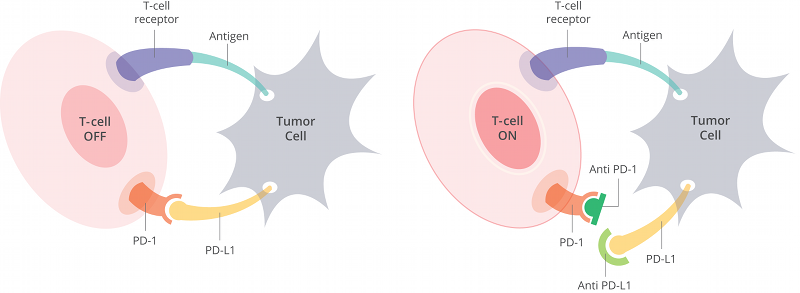
\includegraphics[width = 0.9\textwidth]{Images/pd1-pathway-cb3f6ea987e660555dd535e0223a6a05.png}
    \caption{Mechanism of PD-L1 in checkpoint blockade inhibition in cancer immunotherapy. Figure was adapted from https://www.smartpatients.com/targets/pd-1}
    \label{fig:PDL1_schematic}
\end{figure}




While checkpoint blockade inhibition has enabled cancers of some patients to be treated and eliminated, more than 60\% of patients were found to refractory to this new standard of care in melanoma, a cancer of the skin \cite{ribas2016association}.  To determine mechanisms for cancer immunothereapy resistance, a number of groups had performed high-throughput screens to identify gene targets that sensitizes cancer cells to cancer immunotherapy, leading to the discovery of a large number of targets like Ptpn2 and chromatin regulators \cite{patel2017identification, manguso2017vivo, pan2018major}. However, given the large number of targets identified from these studies, such data sets are difficult to interpret directly. In addition, the relative importance of each of these genes within the biological network is difficult to establish. Thus, better knowledge of the biological networks that underlie checkpoint inhibition, and how they might govern resistance would certainly greatly improve our understanding of how resistance to checkpoint inhibition occurs.

Biological networks describe the relationship between different genes and proteins. When full knowledge of the biochemical networks that underlie these network, including how their interact, and the chemical constants describing these processes are known, one can easily predict the effect of perturbing one gene on the other components of the biological networks. However kinetic parameters describing these biochemical networks are often unavailable, with only knowledge of the topology of these biological networks typically known. Interestingly, a recent study had highlighted how knowledge of the network topology alone was sufficient for attaining a 65–80\% accuracy in predicting the impact of perturbation patterns \cite{SantoliniE6375}, thus enabling the large number of topology based networks which are currently available to be utilized for the study of a large range of biological processes. In particular, the study developed three topology based approaches - Propagation, Distance, and First Neighbours (Section \ref{Numerical_methods}) for inferring the impact on the network on gene perturbation. 

Given that detailed kinetic parameters describing biological pathways determining checkpoint blockade inhibition is lacking, we ask if the topology based approaches introduced in this previous study is sufficient for us to make predictions that are concordant with experimentation. In addition, the agreement between a less complex network model with a more detailed model would also be assessed. Overall, the results would enable us to garner a better understanding of the mechanisms underlying cancer immunotherapy resistance.


\begin{figure}
    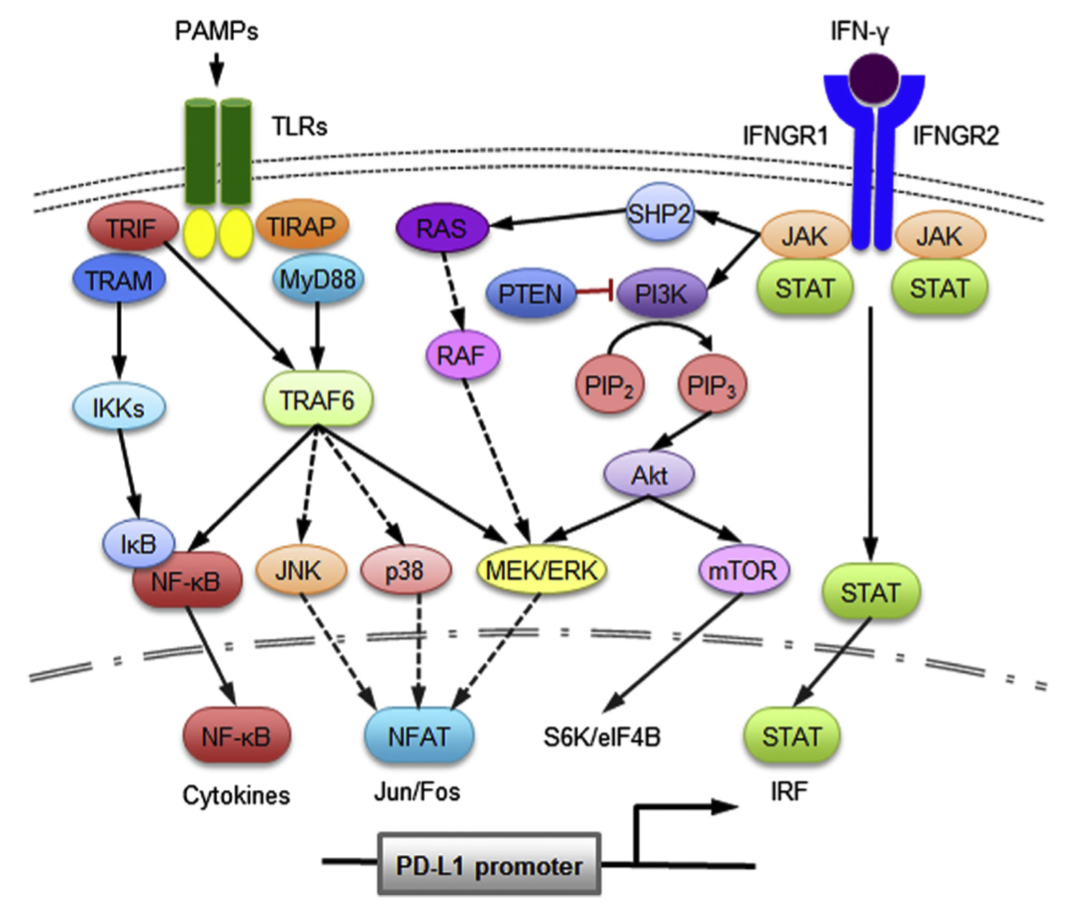
\includegraphics[width = 0.9\textwidth]{Images/PD-L1_pathway.png}
    \caption{Biological pathway depicting genes that regulates PD-L1 expression. Figure was extracted from Ritprajak et al \cite{ritprajak2015intrinsic}}
    \label{fig:PDL1_biologicalpathway}
\end{figure}



\section{Datasets}
\subsection{PD-L1 pathway}

We extracted the PD-L1 pathway which was published by Ritprajak et al \cite{ritprajak2015intrinsic} and also depicted in Figure \ref{fig:PDL1_biologicalpathway}. We then manually curated the pathway and introduced nodes and edges linking each of components in the network. Specifically, when genes form a co-complex for activation of downstream pathways, a ghost node was introduced to represent the co-complex. This co-complex was then linked to downstream components. In addition, we also noted cases in which certain genes indicated in this schematic was represented by multiple degenerate components. In this case, we again created a ghost node to represent the degenerate component, with  constituent components pointing towards this generic component (e.g. STAT1 and STAT5 to the generic component STAT5). Overall, this allowed us to generate the network as observed in Figure \ref{fig:PDL1_network}.


\begin{figure}
    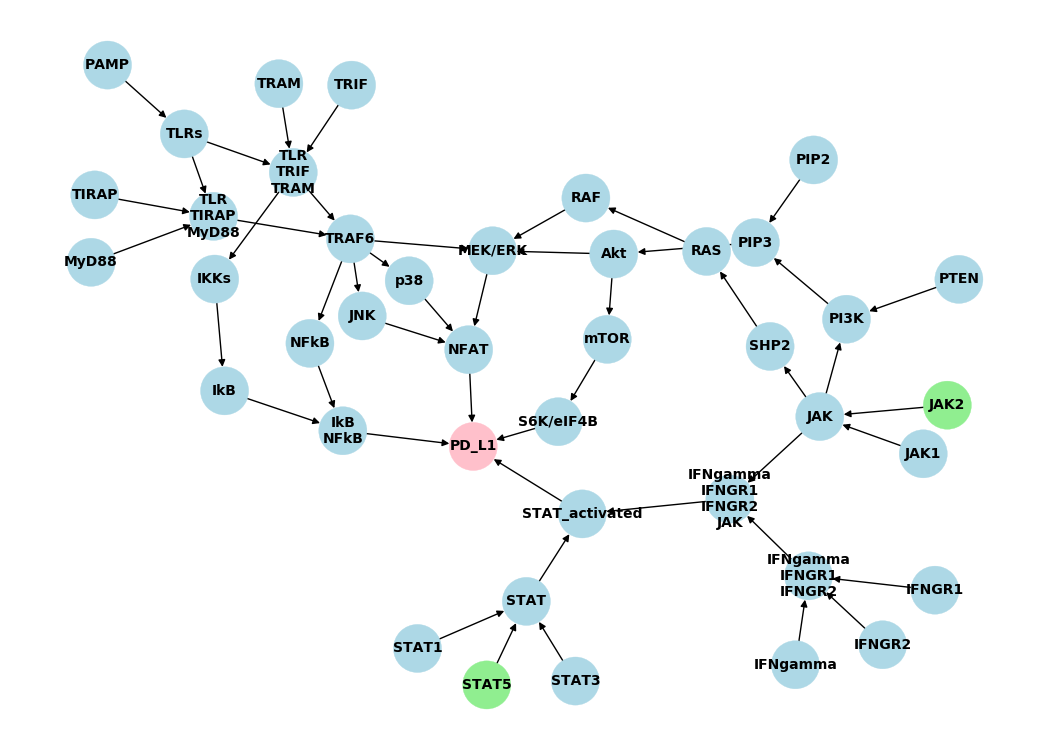
\includegraphics[width = 0.9\textwidth]{Images/PD-L1_pathway_graphViz.png}
    \caption{PD-L1 network generated from the PD-L1 biological pathway. The genes that were perturbed in this study are highlighted in green and the PD-L1 gene is highlighted in pink.}
    \label{fig:PDL1_network}
\end{figure}

\subsection{Gene expression data}
Two previously published gene expression datasets were utilized to determine the impact of gene perturbations on PD-L1 expression, and possible impact on immunothereapy response. Specifically, JAK2 knockdown (GSE54645), and STAT5 knockdown (GSE68993) datasets were utilized for this study. Gene expression datasets were downloaded in R using the GEOquery library in Bioconductor (cite). The probeset information for each dataset was similarly downloaded using GEOquery. Gene names were then annotated using the probeset information. Where gene names information were not available, gene symbols were annotated by comparing the chromosome, start, end, and strand information in the probeset to the UCSC known gene annotations.


\subsection{Genes that confer resistance to immunotherapy from CRISPR knockout screens}

The list of genes that confers sensitivity to cancer immunotherapy, as identified from CRISPR knockout screens, were extracted from three different publications \cite{patel2017identification, manguso2017vivo, pan2018major}. These genes were then manually curated and compared against the list of genes in our biological network and pathway.


\section{Numerical Methods} \label{Numerical_methods}
\subsection{Validating the influence networks}
We first evaluated Santolini's ~\cite{SantoliniE6375} approach against an existing BioModel  (BIOMD0000000313) from the BioModels Database  ~\cite{BioModels2010, PMID:21127196} an IL-13 pathway involving PD-L1. Using the provided code, we converted this BioModel into a Matlab function which represents a system of ODEs. The database also provided a steady state. 

To verify this numerical steady state - we tried both numerically solving the steady state via non-linear equation solving, as well as running an ODE solver (45, 23) and comparing the results. A direct, non-linear solver proved numerically unstable while the ODE solver seeded at the provided steady state matched closely with the database provided value. 

For the influence networks (labeled DYNAMO or dynamical-agnostic models) we implemented 3 classes of models found in the original study (Figure ~\ref{fig:dynamo}). For each of these networks we compute a specific Sensitivity matrix - a square matrix, where the $(i, j)$ component represents the influence of component $j$ on quantity $i$. This sensitivity matrix can then be used to make predictions of the direction of a perturbation (the sign of the $(i, j)$ entry) as well as the relative strength (the absolute value of the entry) ~\cite{SantoliniE6375}

The classes of models are: 
\begin{itemize}
    \item Propagation networks. From an adjacency matrix, $A$, we construct degree matrices. $D_1$ and $D_2$. $D_1$ is a diagonal matrix where the $i$th component is the sum of all the in-degrees for node $i$ and for $D_2$ the $i$th component is the sum of the out-degrees of node $i$
    We then compute the normalized weight $W = D_1^{\frac{-1}{2}}A D_2^{\frac{-1}{2}}$ where $D_1^{-\frac{1}{2}}$ is simply $\frac{1}{sqrt{d_{ij}}}$
    
    (since $D_1$ is just a diagonal matrix ). To compute the sensitivity matrix, we calculate $S = (1 - \alpha)(I - \alpha W)^{-1}$ with $\alpha = 0.9$
    
    \item Distance matrices: Define matrix $D$ where $D_{ij}$ as the number of edges needed to go from $i$ to $j$. The Sensitivity matrix is then the inverse of the distance - more specifically $S_{ij} = 1/(1 + D_{ij})$
    
    
    \item First neighbor: A simple adjacency network as the sensitivity matrix.
\end{itemize}


\begin{figure}
    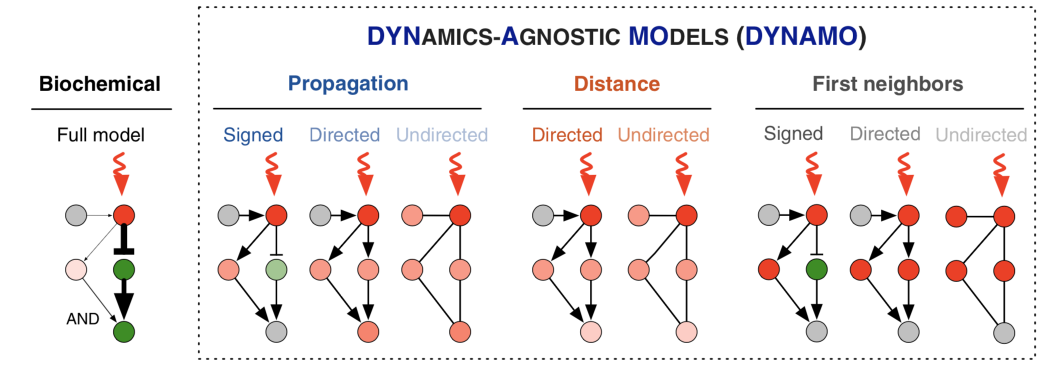
\includegraphics[width = 0.9\textwidth]{Images/dynamo.png}
    \caption{Illustration of biochemical network models, and the propagation, distance, and neighbour topology based network models}
    \label{fig:dynamo}
\end{figure}


The propagation networks can come in the form of a signed directed networked (aware of whether the species up or down regulates) a unsigned directed network (knowledge of the direction of regulation up-regulates or down regulates) or a unsigned undirected networks (knowledge that $A$ and $B$ interact but no direction)

We re-implemented this method in python (see supporting code) to solve the various sensitivity matrices for the different models.

In addition - we decided to try two other approaches for comparisons sake
\begin{itemize}
    \item Eigenvectors of the adjacency matrix. 
    \item Katz-centrality scaled. Here we computed the Katz centrality for each node, and then applied this weighting factor to the adjacency matrix. The Katz centrality of a node can be define as $C(x_i) = \alpha \sum A_{j, i} C(x_j) + \beta$ where $\beta$ is some bias term. This can be written as a matrix eigenvector problem, where we have $C = \alpha A^T C + \beta \textbf{1}$. Solving this out we have $C = \beta(I - \alpha A^T)^{-1} \textbf{1}$ Because of the inverse involved - most solvers (including the one we use) instead use a power iteration to calculate this value. Once we have the centrality values of each nodes, we scale the adjacency by the centrality. In effect this creates a first neighbor model, where the value of of a neighbor of node $i$ is scaled by the centrality score. 
\end{itemize}

In both these cases we computed the sensitivity matrix using the same formulas as the propagation network ($S = (1 - \alpha)(I - \alpha W)^{-1}$ where $W$ is either the eigenvectors or the Katz weighed neighbors. We believe that these models may also perform well because they encode some information about the "global" influence (ex: page-rank like approach) may prove to be an interesting comparison. Katz centrality in particular has been shown to be a good predictor in neuron firing rates and perhaps similar dynamics may be found. ~\cite{doi:10.1142/S0129065717500137}
 
To evaluate these proposed models - we employ two different statistics to test both the accuracy of the "strength" of influence as well as the direction. To test the direction, we simply looked at the signs of the different similarity matrices and check to see how many components are matching. To test the strength, we employ the Spearmans rank correlation coefficient on the absolute value of the various sensitivity matrices. By doing so, we can observe whether the relative ordering of predicted strength of an interaction is preserved across the biochemical model and the newly proposed ones. We consider the absolute value of the coefficients in order to isolate the analysis of the strength of the correlations from the direction.  



\subsection{Evaluating on less understood network}
In order to see whether this analysis could work in a more complex system - a published path - but one without dynamical information known, we performed further analysis using the PD-L1 biological network extracted from a recent publication \cite{ritprajak2015intrinsic}.  Figure ~\ref{fig:PDL1_network} shows the relationship between the various components. Compared to the known BioModel pathway - it is significantly more complex and sparse. 

Using JAK2 knockout data, we computed the various influence models as described in the previous sections. To define the directional changes - we looked the change in mRNA expression from experimental to control for various genes. if the change in expression was more than $10\%$ we consider it to be up-regulated. Any change in expression down $10\%$ or more was considered down-regulated. Values outside of that range were labeled as unchanged. To evaluate the accuracy of the strength prediction - we employed Spearman to see if the rank ordering of the strengths predicted by the influence models were similar the experimental data. Similar analyses were also performed using a STAT5 knockdown dataset.

For the PD-L1 test, we then compared the list of genes that were predicted to cause PD-L1 downregulation, and thus sensitivity to cancer immunotherapy to a number of recent studies. These studies had utilized whole genome CRISPR knockout screens to identify genes that cause cancerous cells to be more sensitive to these therapeutics. Indeed, if PD-L1 is predicted to be down-regulated in our network, then it should confer cancerous cells sensitivity towards checkpoint blockade cancer immunotherapy as is observed in these experiments.
\section{Results}

\subsection{Biomodel}

Figure ~\ref{fig:biomodel_res} shows the result of the Biomodel comparison. Looking at the correlations in Figure  ~\ref{fig:unsigned_correlation_biomodel} we see that we see that the propagation network, both respecting direction with one respective sign and the other one not - perform reasonably well (0.9 and above). A directed distance method also performed fairly well. Interestingly enough, an approach based on the sensitivity of the eigenvectors performed poorly but an approach based on Katz sensitivity performs extremely well.  

Figure ~\ref{fig:percent_agreement_biomodel} shows the percent agreement in sign across the various model. Here we see that the signed propagation network and the distance metric performs reasonably well. The fact that the unsigned metrics also perform relatively high suggests that the incremental improvement in having a signed understanding is relatively marginal (around 0.15 correlation pickup) - suggesting that this network was fairly one directional to start with. Interestingly the Katz based approach performed fairly poorly in predicting the sign while doing well at predicted strength. 



\begin{figure}
    \centering
    \begin{subfigure}[b]{0.45\textwidth}
        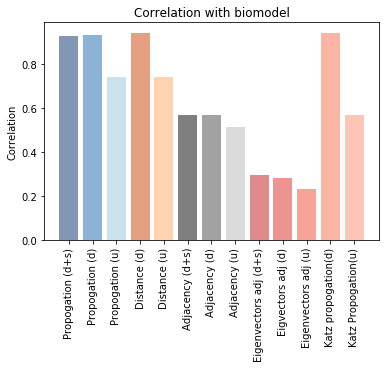
\includegraphics[width=\textwidth]{Images/Correlation_unsigned_biomodel.png}
        \caption{Spearman correlation between the given model and the full biochemical model}
        \label{fig:unsigned_correlation_biomodel}
    \end{subfigure}
    ~ %add desired spacing between images, e. g. ~, \quad, \qquad, \hfill etc. 
      %(or a blank line to force the subfigure onto a new line)
    \begin{subfigure}[b]{0.45\textwidth}
        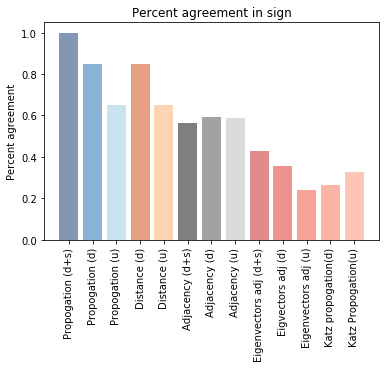
\includegraphics[width=\textwidth]{Images/Percent_agreement_direction.png}
        \caption{Sign agreement between the given model and the biochemical model }
        \label{fig:percent_agreement_biomodel}
    \end{subfigure}
    \caption{Results of comparing biochemical model with the the various influence networks  (propagation networks -blue, distance - orange, First neighbors - grey, eigenvector based - red}  
    \label{fig:biomodel_res}
\end{figure}

\subsection{Jak2 experimental verification}

For the JAK2 knockdown comparison (which we limited to just the 3 classes of models originally proposed), the correlations are, however, significantly worse. In Figure ~\ref{fig:JAK2_strength} we see that the highest correlations are $0.25$  with the Propagation (d + s) network. The sign agreement performs slightly better in figure ~\ref{fig:JAK2_percent} where the top performing models (signed propagation, unsigned directed and distance) predicted roughly $70\%$ of the directional.

We hypothesize the poor performance of the correlation may come due the differing natures of the networks - the BIOMODEL's networks and most models in that repository tend to be smaller (fewer nodes) and more connected (more edges) - which may imply that the localized network is relatively well understood. There's a partial selection bias as well - the BIOMODEL's networks had have to been extremely well studied to come up with rate constants in the first place, while in comparison - a pure topology network may not have the same level of detail. 


\begin{figure}
    \centering
    \begin{subfigure}[b]{0.45\textwidth} 
        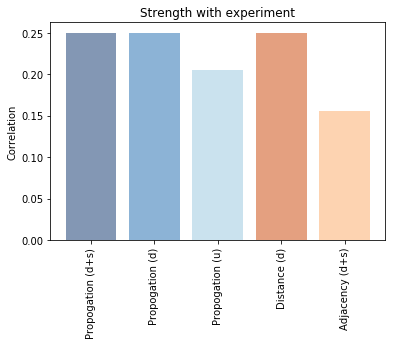
\includegraphics[width=\textwidth]{Images/Experiment_Jak2_correlation.png}
        \caption{Rank correlation result relative to RNA expression. RNA expression data was compiled for various genes in relation to a knockout of JAK2. The sensitivity matrices were then computed for the various method, and the rank correlations were computed to understand whether relative strengths were being captured}
        \label{fig:JAK2_strength}
    \end{subfigure}
    ~ %add desired spacing between images, e. g. ~, \quad, \qquad, \hfill etc. 
      %(or a blank line to force the subfigure onto a new line)
    \begin{subfigure}[b]{0.45\textwidth}
        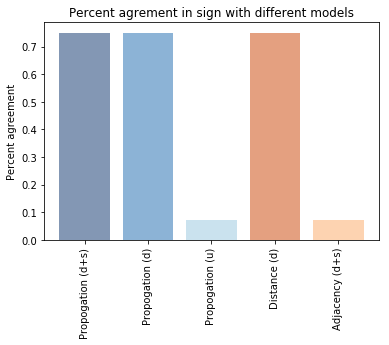
\includegraphics[width=\textwidth]{Images/Experiment_Jak2_sign.png}
        \caption{Percent agreement in sign relative to RNA expression. In the JAK2 knockout, an increase of above $10\%$ corresponded to a $1$ for comparison purposes, below $10\%$ resulted in a $-1$ and everything else $0$. This was compared to the corresponding output in the sensitivities matrices of various models}
        \label{fig:JAK2_percent}
    \end{subfigure}
    ~ %add desired spacing between images, e. g. ~, \quad, \qquad, \hfill etc. 
    %(or a blank line to force the subfigure onto a new line)
    \caption{Results of Jak2 knockdown experimental verification}  
\end{figure}

\subsection{Stat5 experimental verification}
Stat5 experimental verification was also performed using a Stat5 knockdown dataset (GSE68993). However, there was a relatively poor overlap between genes present in this dataset, with genes in our manually curated biological pathway. The results of the analysis were thus not very informative, and not presented here.


\subsection{PD-L1 experimental validation}
To determine if topology based networks utilized in our study is able to make prediction of genes that confer resistance to cancer immunotherapy, we computed the sensitivity matrix of the various models and ask if the results are concordant with experimentally defined list of genes that confer resistance to cancer immunotherapy. We first artificially down-regulated the expression of each node, and then assessed the expression of PD-L1 following gene perturbation (Figure \ref{fig:heatmap}). Notably, our network indicate that PD-L1 expression remains unchanged when most of the genes are perturbed. These results were also observed across different types of models (Propagation, Distance, neighbours). Only in the 'Distance - unsigned model' was the PD-L1 expression predicted to decrease in all cases.

 Interestingly, our model predicted that down-regulation of mTOR, PIP2, Akt, and NFAT to have a strong impact on PD-L1 downregulation (Figure \ref{fig:heatmap}). However, only the AKT genes (AKT1, AKT2, AKT3) were identified in these experimental studies (Figure \ref{fig:comparisonHits}). Conversely, many more weak candidates identified in our network were identified in these three studies. Nonetheless, we also note poor concordance between these 3 experimental studies. Thus, the poor concordance of our topology based methodology with these studies may be due to a lack of sensitivity and/or specificity of theses original experimental studies.

\begin{figure}
    \centering
    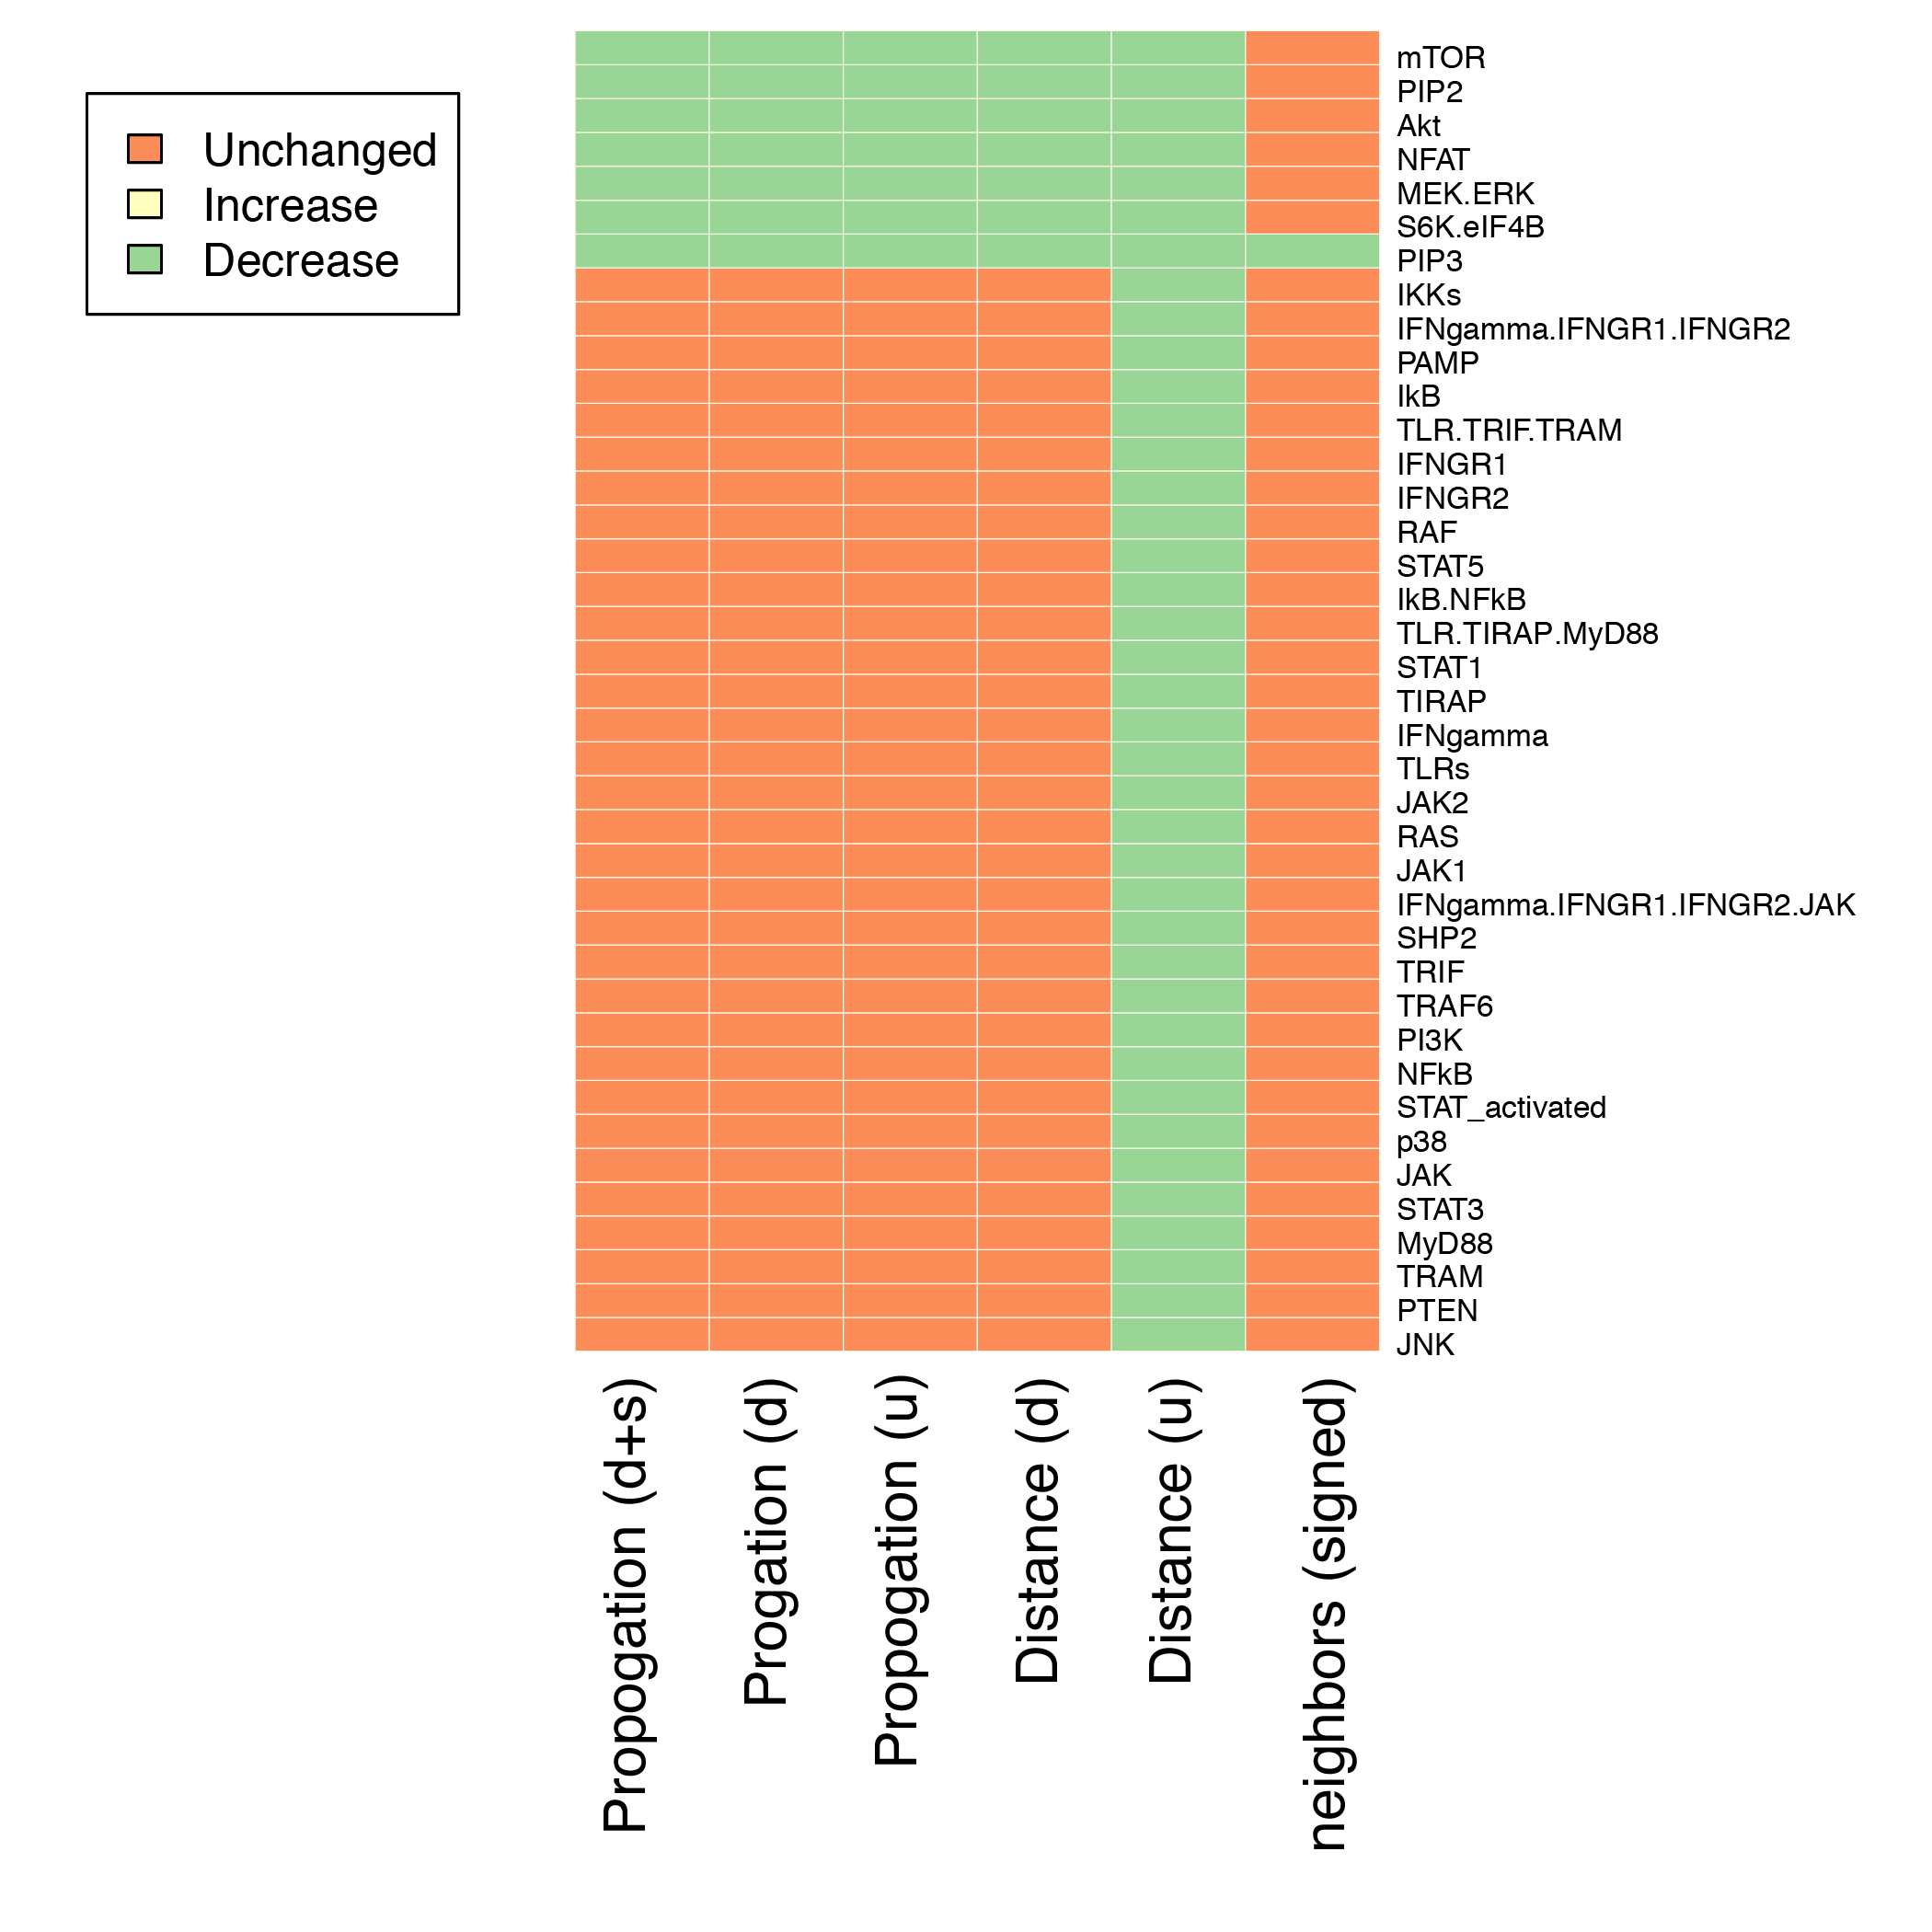
\includegraphics[scale = 0.8]{Images/heatmap_clean-01.png}
    \caption{Predicted impact of down regulation of each gene on PD-L1 gene expression, using different topology based network approaches.}
    \label{fig:heatmap}
\end{figure}


\begin{figure}
    \centering
    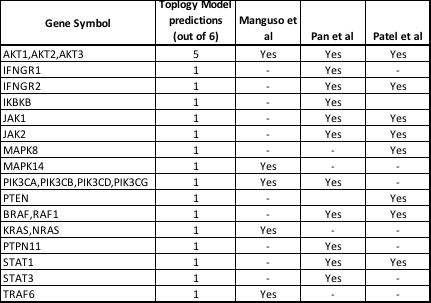
\includegraphics[scale = 0.8]{Images/ComparisonHits.png}
    \caption{Comparison of genes that are predicted to confer sensitivity from topology networks, with genes that are identified from three different studies. Genes that were found found to confer sensitivity to cancer immunotheraepy were labelled with a "Yes"}
    \label{fig:comparisonHits}
\end{figure}





\subsection{Limitations}
While the evaluation on the biomodel seemed to perform reasonably well, the performance on the PD-L1 model against expression data did not perform as well. We postulate several possible reasons: 
\begin{itemize}
    \item Systems difference - while the original models were tested primarily on bacterial systems, mammalian systems display a much more complex regulatory network - which may necessitate knowing more dynamical information that a simple topology approach may have. 
    \item Less information about the system. Systems that already kinetic rate constants by their nature would be far better understood than a system that doesn't. There may be parts in the PD-L1 pathway that we still do not fully grasp. 
    \item mRNA expression data utilized in this study is a proxy for protein expression. However, proteins levels which truly govern the biochemical networks may not be properly represented by mRNA expression. Utilization of protein expression data, like those collected using mass spectrometry is more likely to yield more meaningful results.
\end{itemize}

\section{Conclusions and future works}
While the topology based dynamic approach sounded appealing, when evaluating against these larger, more complex networks than the ones original studies, it becomes less clear. When evaluating against expression data, directional outcomes could be well predicted but not strength. When evaluating predicted impact on PD-L1, the various models predicted many more interactions than what was observed. It may be difficult to say whether it was a short coming in those studies or our models, but based on initial evidence, it is hard to conclude if these topology based dynamical networks could be used. Further studies on mTOR, PIP2, and NFAT relationship with PD-L1 would help verify or refute our model's predictions. In addition, mRNA as a proxy may not fully capture the protein protein 

One bright spot that would be exploring further would be evaluating further the Katz's based models - in particular their incorporation of signed network in some fashion may help in improving the sign prediction accuracy. Further eigenvector based approach's may field similarly interesting results. 



\section{Appendix}
The github can be found at https://github.com/ktan8/AM205-Project

\bibliographystyle{plain}
\bibliography{references}
\end{document}
